\documentclass[a4paper]{article}
\usepackage[french]{babel}
\usepackage[utf8]{inputenc}
\usepackage[T1]{fontenc}
\usepackage{graphicx}   % pour les images
\usepackage{hyperref}   % pour les références
\usepackage{amssymb}    % pour les symboles de maths comme \mathbb{R}
\usepackage{mathtools}  % pour rajouter \text dans un environment math
\usepackage{subcaption} % pour les subfigures
\usepackage{float}      % pour les figures

\usepackage[backend=biber]{biblatex}
\addbibresource{ref.bib}
% \usepackage[style=ieee]{biblatex}
% \addbibresource{ref.bib}
% \bibliography{ref.bib}

\hypersetup{
    colorlinks=true,
    linkcolor=blue,   % Couleur des liens internes (table des matières, références)
    citecolor=green,  % Couleur des liens vers les références bibliographiques
    filecolor=magenta,% Couleur des liens vers les fichiers
    urlcolor=blue     % Couleur des liens vers les URL
}

\title{Rapport SAM \\ Modèle multi-modaux}
\author{Cléa Han, Yanis Labeyrie et Adrien Zabban}
\date{janvier 2024}

\begin{document}

\maketitle

\section{Introduction}

Notre projet traite des approches multimodales pour la prédiction de changement de prise de parole dans des conversations naturelles. 
Nous nous appuyons sur le corpus de données multimodales appelé Paco-Cheese.
Les objectifs de ce projet nous permettent d'introduire différentes notions de modalité textuelle, visuelle et auditf, ainsi que de
comparer et d'explorer différents modèles de traitement multimodaux, et leur fusion entre eux.

\section{Données}

Les données proviennent d'un ensemble de données multimodales, en français, composé de 26 dyades de 15 à 20 minutes.
Chaque dyade est composée de deux personnes qui discutent d'un sujet donné. Les données sont composées de trois modalités : la vidéo,
l'audio et le texte.
Dans le cas des vidéos, les données sont déjà pré-traitées et sont composées de landmarks du visage des deux personnes en conversation. 
Ces données sont des séquences de 10 images par personne, soit 20 images au total. Les données audio sont des enregistrements audio
des deux interlocuteurs. Enfin, les données textuelles sont des scripts de conversation des deux interlocuteurs.
En effet, les données sont annotées de deux manières : avec de la segmentation de la parole basée sur les silences en utilisant les
IPUs et avec des scripts de conversation, qui servent eux le traitement de texte. 
Les IPUs (Inter-Pausal Units) représentent des segments de parole séparés par des pauses de paroles et sont utilisés comme unité de
parole dans l'analyse de conversations.
Utiliser l'unité du IPU permet d'analyser la structure et le rythme de la dynamique conversationnelle. 

Au-delà des fichiers audios et des fichiers textes qui sont sous leur format traditionnel respectif, 
les données des vidéos seront traitées à travers de fichier csv qui contiennent les landmarks du visage des deux personnes en
conversation. Ces fichiers csv sont composés de colonnes indicant les caractéristiques des différentes prises de paroles. 

Ces données "vidéos" sous forme de fichiers csv causent une significative augmentation du temps de chargement de ces données étant
donné qu'ils donnent le lien vers des ressources à charger, et ce pour chaque ligne du fichier csv. 
Pour palier ce problème, nous avons utilisé des \textit{skiprows} afin d'en accélérer le processus et de sélectionner les données
pertinentes à notre apprentissage.

\section{Traitement unimodale}

\subsection{Traitement du texte avec CamemBERT}

Pour parvenir à détecter le changement de tour de parole dans les données textuelles, nous avons choisi d'utiliser un modèle
considéré comme l'état de l'art pour la tâche de classification de texte : le modèle BERT (Bidirectional Encoder
Representations from Transformers~\cite{Bert}). Ce modèle utilise notament les Transformers~\cite{transformers} (voir Figure~\ref{fig: Transformers}).

Par ailleurs, BERT étant un modèle comprenant un nombre important de paramètres (environ 100 millions) il est inenvisageable avec
nos moyens de l'entraîner "à partir de 0". Nous avons donc opté pour l'utilisation d'un modèle pré-entrainé sur la langue Française
appelé CamemBERT et nous avons gelé les poids de CamemBERT.

\begin{figure}[H]
    \centering
    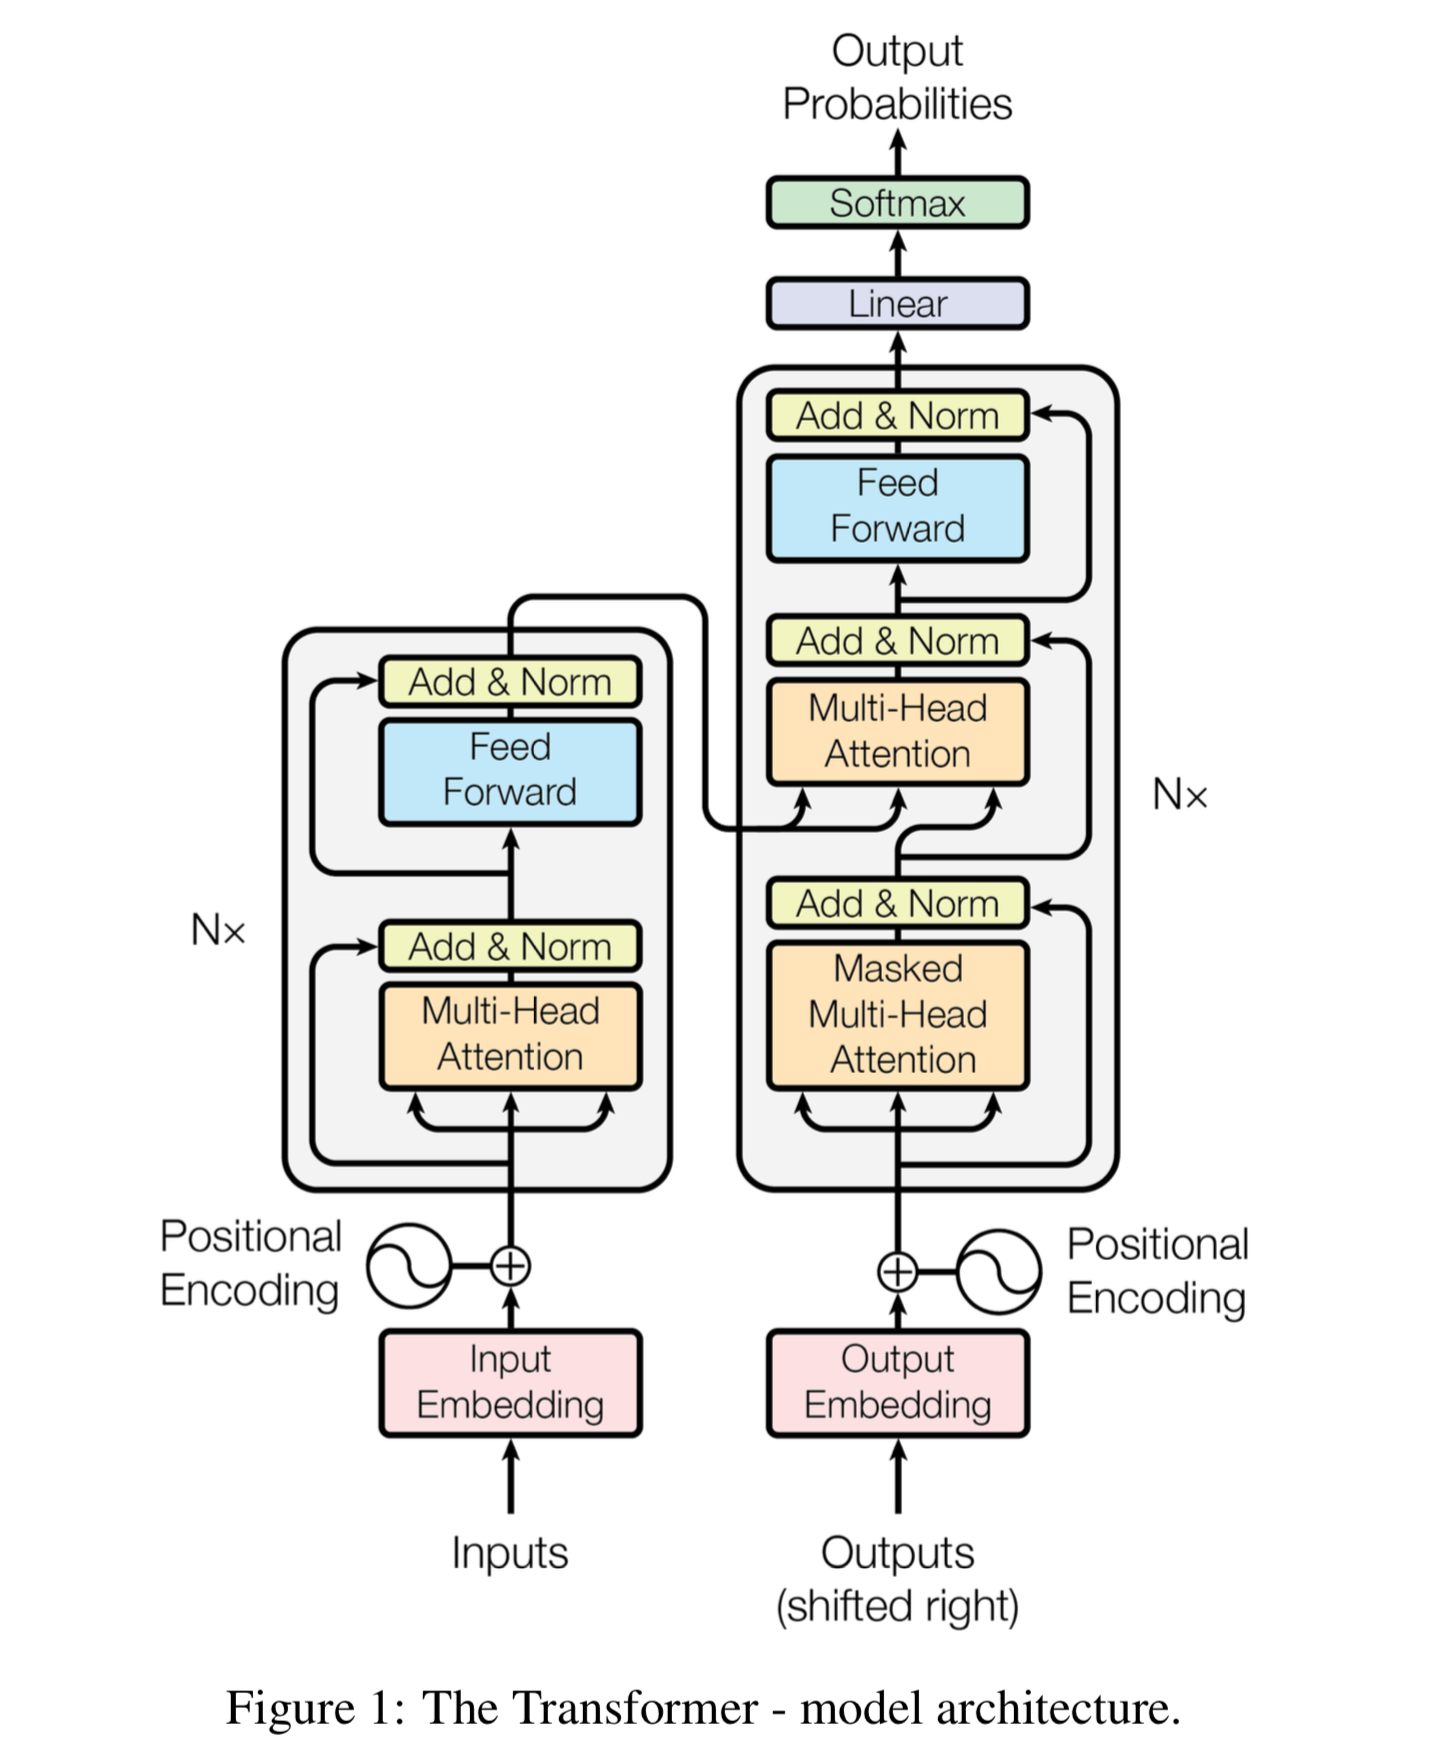
\includegraphics[width=0.6\textwidth]{model_transformers.png}
    \caption{Architecture de Transformers}
    \label{fig: Transformers} 
\end{figure}



On prend alors les données de textes qui sont une liste d'entiers, correspondant 
à l'indice de chaque mot du tokenizer de CamemBERT. Ces données passent alors dans CamemBERT, elles ressortent avec une dimension de
768. Elles passent alors dans une activation ReLU puis une couche dense de taille 768, puis une couche de dropout (avec un taux
d'oublie de $10\%$), pour enfin passer un dernier ReLU et une dernière couche dense à 2 dimensions. 
La Figure~\ref{fig: model_text} résume l'architecture de ce modèle, qu'on appelera \textit{TEXT}.

\begin{figure}[H]
    \centering
    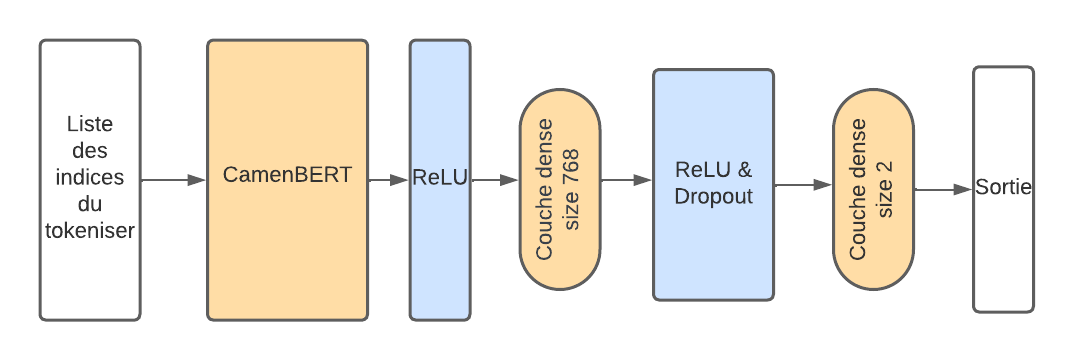
\includegraphics[width=0.6\textwidth]{model_text.png}
    \caption{Architecure du modèle \textit{TEXT}.}
    \label{fig: model_text}
\end{figure}

\subsection{Traitement de l'audio}

Afin de détecter les changements de parole dans des données audio, nous avons choisi d'exploiter une approche similaire en utilisant
un modèle avancé dans le domaine de la représentation audio : le modèle Wave2Vec~\cite{wav2vec}. Wave2Vec, basé sur les Transformers, s'est établi
comme une référence pour la tâche de traitement du signal audio, en particulier pour la détection des variations dans la parole.
Grâce à sa capacité à encoder de manière bidirectionnelle les représentations des signaux sonores, Wave2Vec excelle dans la
compréhension des nuances acoustiques et des transitions subtiles entre les locuteurs. 

On possède deux données en entrée qui sont les enregistrements audio des deux interlocuteurs. On fait alors passer leurs audio dans
Wave2Vec puis l'on concatène la sortie. On fait alors passer la concaténation dans une couche dense pour n'avoir qu'une sortie de
taille 2.
Eventuellement, ce modèle initial pouvait être amélioré en terme d'architecture, nous avons donc à l'issue de la concaténation,
ajouter une couche dense, puis une couche de ReLU et de dropout, et enfin finir sur une couche dense de sortie à 2 neurones. 
La Figure~\ref{fig: model_audio} résume l'architecture de ce modèle, qu'on appelera \textit{AUDIO}.

\begin{figure}[H]
    \centering
    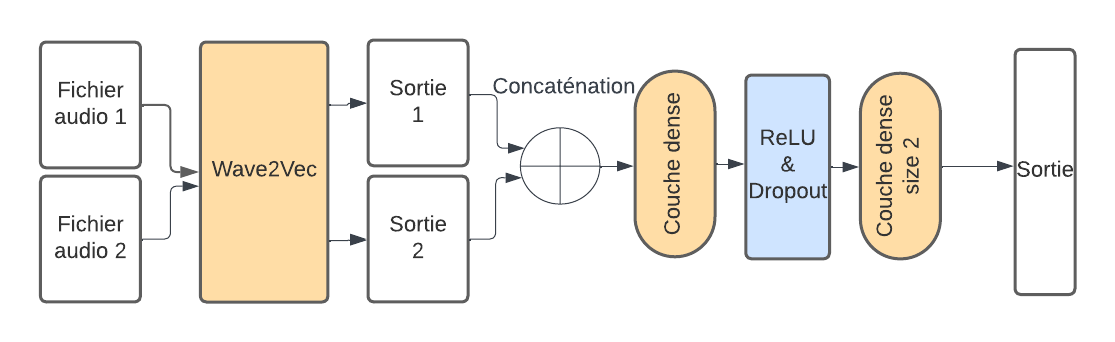
\includegraphics[width=0.6\textwidth]{model_audio.png}
    \caption{Architecure du modèle \textit{AUDIO}.}
    \label{fig: model_audio}
\end{figure}

\subsection{Traitement de la vidéo}

Pour traiter les données issues de la vidéo qui sont sous la forme des landmarks du visage des deux personnes en conversation,
nous avons choisi d'utiliser un réseau de neurones adapté à cette tâche d'analyse de séries temporelles : le réseau LSTM (Long-Short
Term Memory). En effet, ce modèle est pertinent pour la détection du changement de locuteur, car il est capable de conserver des
informations sur de longues séquences temporelles, ce qui est essentiel pour analyser les variations subtiles dans les mouvements
des landmarks faciaux. 

Comme pour l'audio, la vidéo contient un ensemble de deux fois 10 images pour chacun des interlocuteurs. On les fait alors passer
dans deux couches LSTM et on concatène les sorties pour ensuite les faire passer dans du relu et une couche dense de taille 2.
La Figure~\ref{fig: model_video} résume l'architecture de ce modèle, qu'on appelera \textit{VIDEO}.

\begin{figure}[H]
    \centering
    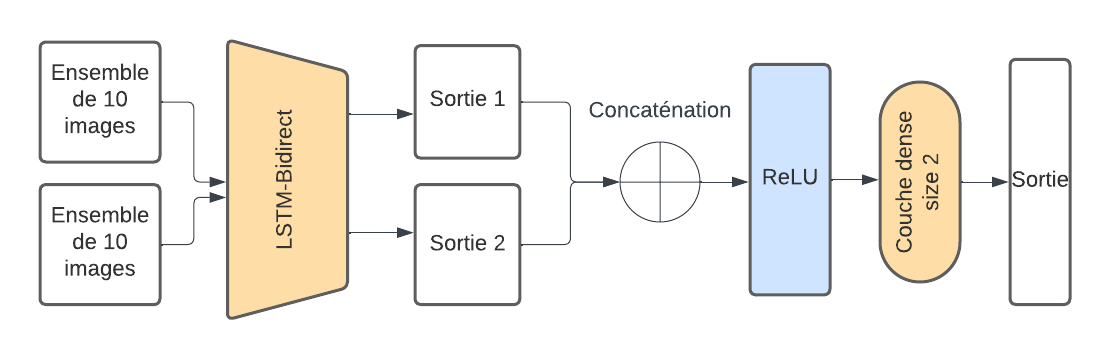
\includegraphics[width=0.6\textwidth]{model_video.png}
    \caption{Architecure du modèle \textit{VIDEO}.}
    \label{fig: model_video}
\end{figure}

\section{Traitement multimodal}

Notre approche vise à maximiser l'utilisation des dépendances et complémentarités entre différents types de données (vidéo, texte,
audio). Pour effectuer des prédictions en utilisant ces diverses modalités, nous avons opté pour l'utilisation de chaque réseau de
neurones présenté précédemment afin d'extraire des représentations compressées (ou features) des différents types de données. 

Les modèles individuels sont initialement pré-entraînés, puis fusionnés en une seule architecture multimodale qui subit ensuite un
nouvel entraînement. Le pré-entraînement des modèles individuels présente l'avantage de réduire le temps de convergence de
l'entraînement de cette architecture multimodale comprenant un nombre important de paramètres.

Au cours de ce processus, pour des raisons de contraintes de ressources, on gèle les poids des modèles unimodales.

\subsection{Maximum de vraisemblance}
Ce premier modèle multimodal fait passer chaque donnée dans son modèle pré-entraîné associé et fait une moyenne des sorties. Le but
est alors de faire une moyenne des probabilités selon chaque canal. Nous appellerons ce modèle \textit{LIKELIHOOD} du fait que le but
est de maximiser la log-likelihood.
La Figure~\ref{fig: likelihood} résume l'architecture de ce modèle.

\begin{figure}[H]
    \centering
    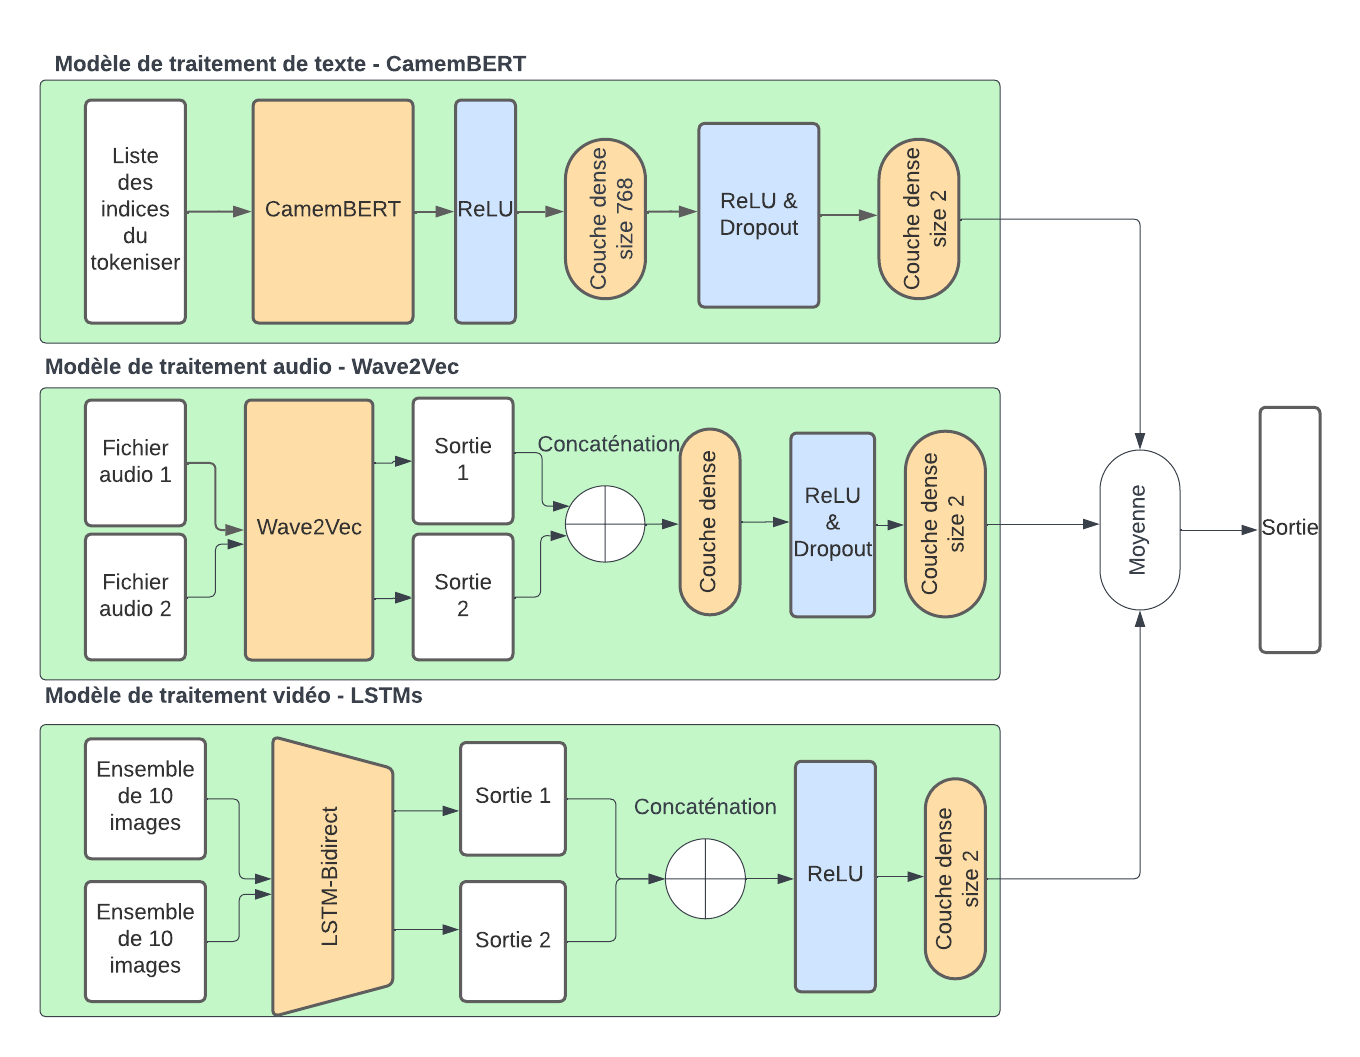
\includegraphics[width=0.6\textwidth]{Likelihood.png}
    \caption{Architecure du modèle \textit{LIKELIHOOD}}
    \label{fig: likelihood}
\end{figure}

\subsection{Apprentissage multi}
Ce deuxième modèle plus évolué consiste à faire passer chaque donnée dans son modèle pré-entraîné associé et de récupérer
l'information avant qu'elle ne passe dans la dernière couche dense (celle de taille deux). On concatène alors toute l'information 
et l'on la fait passer dans une grande couche dense de taille 2.
La Figure~\ref{fig: multi} résume l'architecture de ce modèle, qu'on appelera \textit{MULTI}.

\begin{figure}[H]
    \centering
    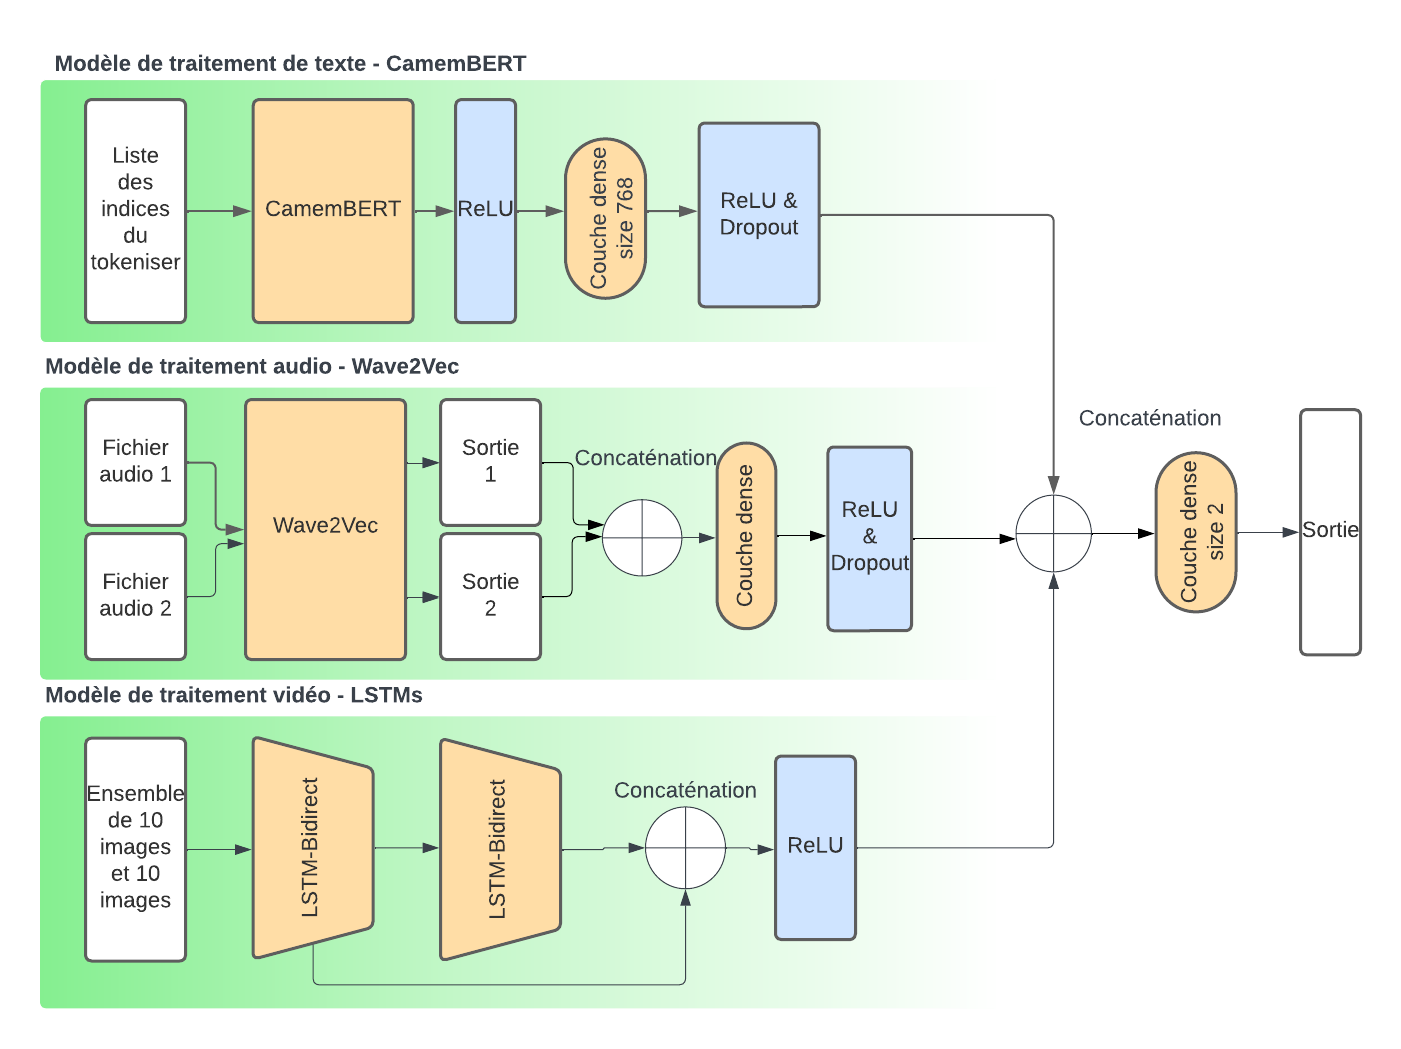
\includegraphics[width=0.6\textwidth]{model_multi.png}
    \caption{Architecure du modèle \textit{MULTI}.}
    \label{fig: multi}
\end{figure}

\section{Results}

\subsection{Métriques}

Pour comparer les résultats obtenu, nous avons utilisé la loss (la crossentropy), mais aussi d'autres métriques,
comme l'accuracy, la précision, le rappel et le $f_1$-score.

\subsection{Uni-modales}

Nous avons entrainé les modèles \textit{TEXT}, \textit{AUDIO} et \textit{VIDEO}. Les deux premier modèles ont 
été entrainé sur 5 epochs. La Figure~\ref{fig: train unimodale} montre la coubres d'accuracy d'entraînement 
et de validation lors de l'entraînement de ces modèles.
Cependant, l'entraînement du modèle \textit{VIDEO}, du a la grandeur des données et 
leurs temps de chargement dans la RAM, nous avons décidé de faire qu'une seule epoch
\footnote{Une epoch durait plus de 2h30 sur google colab avec un GPU Nvidia T4.}.


\begin{figure}[H]
    \centering
    \begin{subfigure}{0.45\textwidth}
        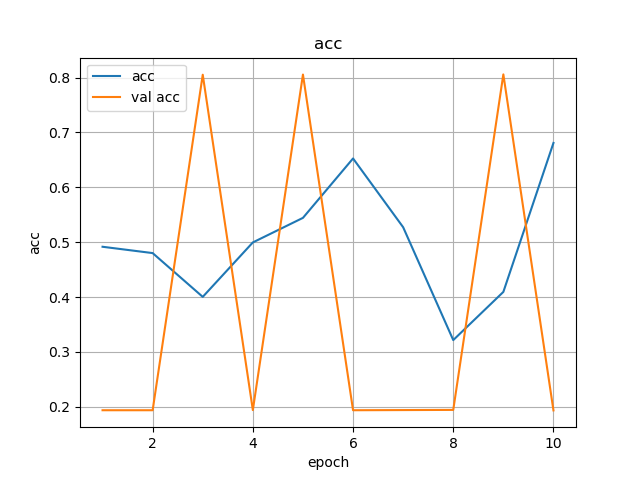
\includegraphics[width=\textwidth]{../logs/text_4/acc.png}
        \caption{Accuracy du model \textit{TEXT}}
    \end{subfigure}
    \hfill
    \begin{subfigure}{0.45\textwidth}
        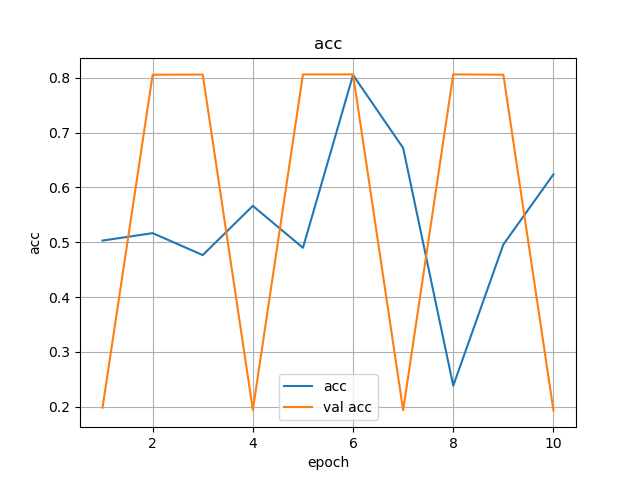
\includegraphics[width=\textwidth]{../logs/audio_2/acc.png}
        \caption{Accuracy du model \textit{AUDIO}}
    \end{subfigure}
    \caption{Courbes d'apprentissage des models uni-modales \textit{TEXT} et \textit{AUDIO} sur l'apprentissage.}
    \label{fig: train unimodale}
\end{figure}

La Table~\ref{tab: test unimodal} présente les résultats des modèles sur le corpus de test.

\begin{table}[H]
    \centering
    \begin{tabular}{|c|c|c|c|c|c|}
        \hline
        Modèle & loss & accuracy & precision & rappel & $f_1$ score\\
        \hline
        \textit{TEXT} & 0.539 & 0.823 & 0.828 & 0.816 & 0.822\\
        \hline
        \textit{AUDIO} & 0.458 & 0.828 & 0.828 & 0.828 & 0.828\\
        \hline
        \textit{VIDEO} & 0.773 & 0.443 & 0.182 & 0.032 & 0.053\\
        \hline
    \end{tabular}
    \caption{Résultats de test des modèles uni-modales}
    \label{tab: test unimodal}
\end{table}

\subsection{Multimodal}

Voici le résultat obtenu pour le modèle multimodal :

\begin{figure}[h]
    \centering
    \begin{subfigure}{0.45\textwidth}
        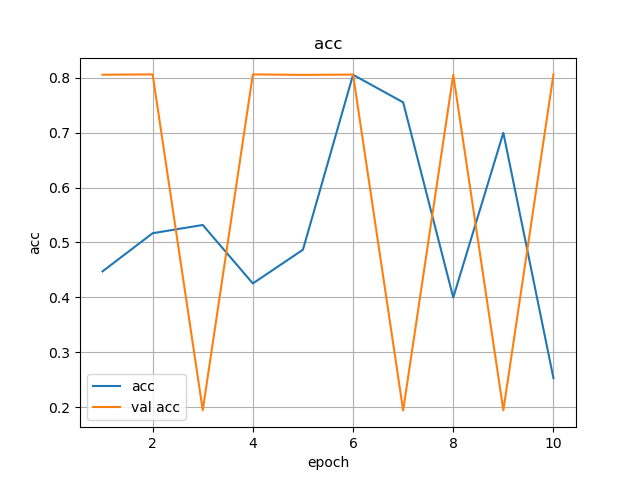
\includegraphics[width=\textwidth]{../logs/multi_3/acc.png}
        \caption{Accuracy of the multimodal model (text+audio) experiment.}
        \label{fig:multi_1_acc}
    \end{subfigure}
    \hfill
    \begin{subfigure}{0.45\textwidth}
        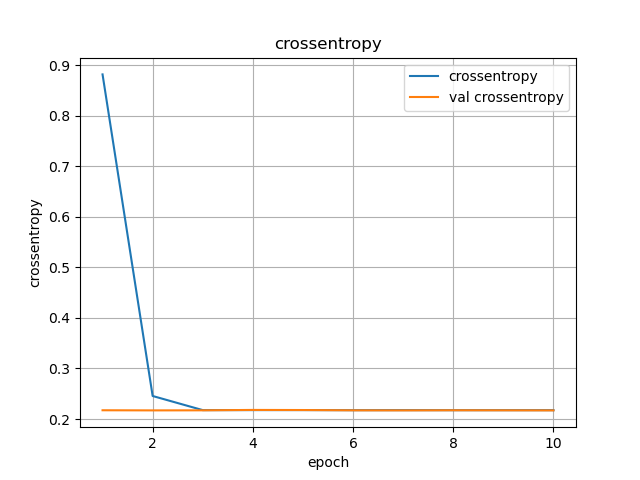
\includegraphics[width=\textwidth]{../logs/multi_3/crossentropy.png}
        \caption{Cross-entropy loss of the multimodal model (text+audio) experiment.}
        \label{fig:multi_1_loss}
    \end{subfigure}
    \caption{Results of the multimodal model (text+audio) experiment.}
    \label{fig:multi_1_results}
\end{figure}

% Les graphiques de la Figure \ref{fig:multi_1_results} présentent les résultats de l'expérience multimodale. L'axe des abscisses
% représente le nombre d'époques, et l'axe des ordonnées représente l'exactitude du modèle pour la Figure \ref{fig:multi_1_acc} et la
% perte en entropie croisée pour la Figure \ref{fig:multi_1_loss}.
% D'après ces graphiques, on peut déduire que le modèle est parvenu à apprendre à prédire les changements de tour de parole en tirant
% parti à la fois des données textuelles et audio.
% \section{Conclusion}

\bigskip
\printbibliography

\end{document}
